% !TEX program = latexmk
\documentclass[aspectratio=169]{beamer}

% ---------- Theme ----------
\usetheme{Madrid}
\usecolortheme{default}

% ---------- Packages ----------
% LuaLaTeX handles Unicode natively — no inputenc/fontenc needed
\usepackage{fontspec}
\usepackage{kotex}          % Korean support (uses luatexko under the hood)
\usepackage{amsmath, amssymb}
\usepackage{graphicx}
\usepackage{booktabs}       % nicer tables
\usepackage{hyperref}

%Added to put subfigures
\usepackage{subcaption}

% ---------- Fonts ----------
% kotex picks a default Korean font automatically.
% Uncomment and change to a specific font if the default is unavailable:
% \setmainfont{Noto Serif}
% \setsansfont{Noto Sans}
% \setmainhangulfont{Noto Serif CJK KR}
% \setsanshangulfont{Noto Sans CJK KR}

% Korean italic workaround:
% CJK fonts have no italic variant, so \textit{} silently does nothing.
% \hangulit applies fontspec's FakeSlant (geometric slant) to simulate italics.
\newcommand{\hangulit}[1]{{\addhangulfontfeatures{FakeSlant=0.167}#1}}

% ---------- Metadata ----------
\title[]{Kaggle로 ML 배우기}
% \subtitle{Subtitle (optional)}
\author[Jaehyun Bhang]{Jaehyun Bhang}
\institute[Inspien / Dev Team]{Inspien / Dev Team}
\date{\today}

% ---------- Document ----------
\begin{document}

\begin{frame}
    \titlepage
\end{frame}

\begin{frame}{Outline}
    \tableofcontents
\end{frame}

% ==================================================
\section{Key Takeaways}
\title[1/4 Key Takeaways]{}
% ==================================================

\begin{frame}{Key Takeaways}
    \begin{itemize}
        \item 개발과정에도 적용가능한 통찰
        \item ML으로 통찰을 얻고 직관력을 키우는 방법
        \item 이런 ML을 노베이스부터 시작하는 방법
    \end{itemize}
\end{frame}

% ==================================================
\section{Why ML?}
\title[2/4 Why ML?]
% ==================================================

\begin{frame}{}
    \begin{figure}[H]
        \centering
        \begin{subfigure} [b] {0.3\textwidth}
            \centering
            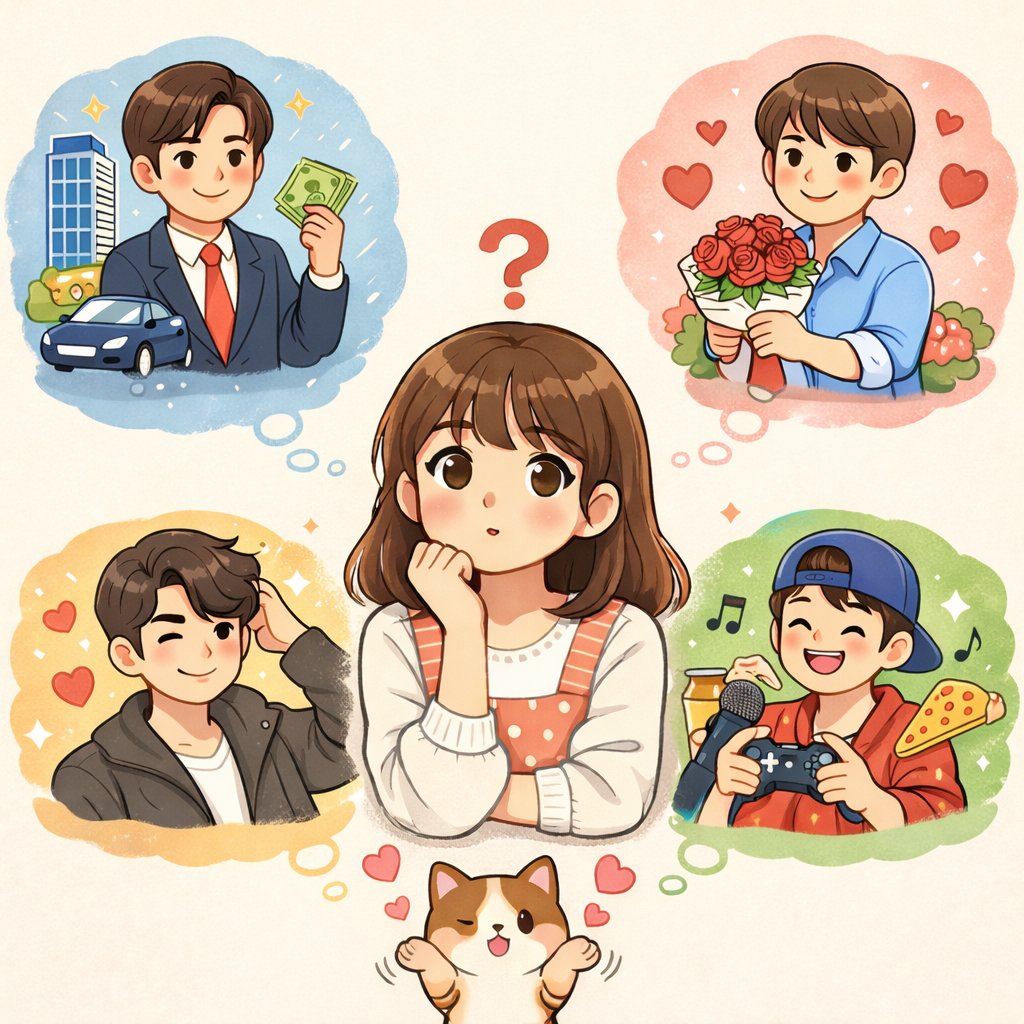
\includegraphics[width=.80\linewidth]{figure/whyML-1.png}
            \caption{}
        \end{subfigure}
        \begin{subfigure} [b] {0.3\textwidth}
            \centering
            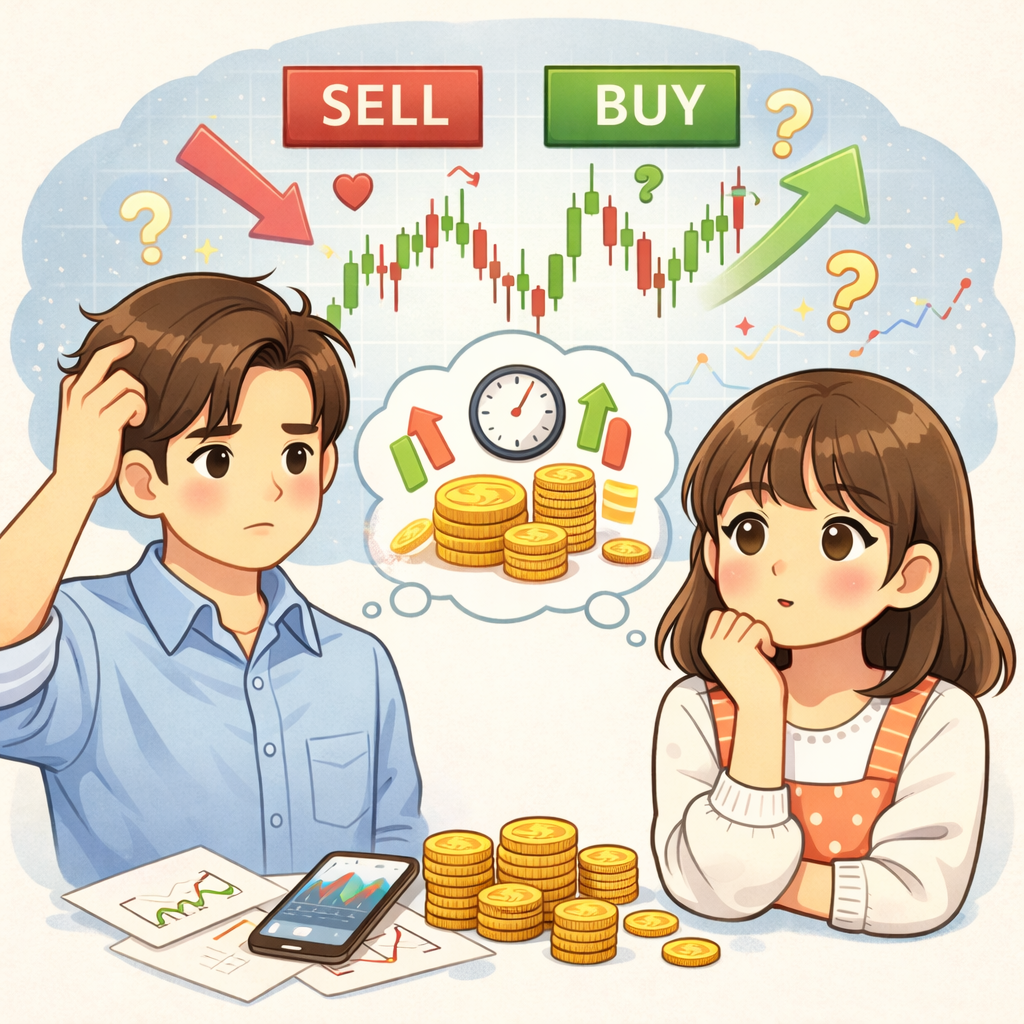
\includegraphics[width=.80\linewidth]{figure/whyML-2.png}
            \caption{}
        \end{subfigure}
        \begin{subfigure} [b] {0.3\textwidth}
            \centering
            
\includegraphics[width=.80\linewidth]{figure/whyML-3.pdf}
            \caption{}
        \end{subfigure}
        % \caption{}
        % \label{fig:vis-comparison}
    \end{figure}
\end{frame}

\begin{frame}{Simple Puzzle (with linear regression)}
    \begin{figure}[H]
        \centering
        \begin{subfigure} [b] {0.47\textwidth}
            \centering
            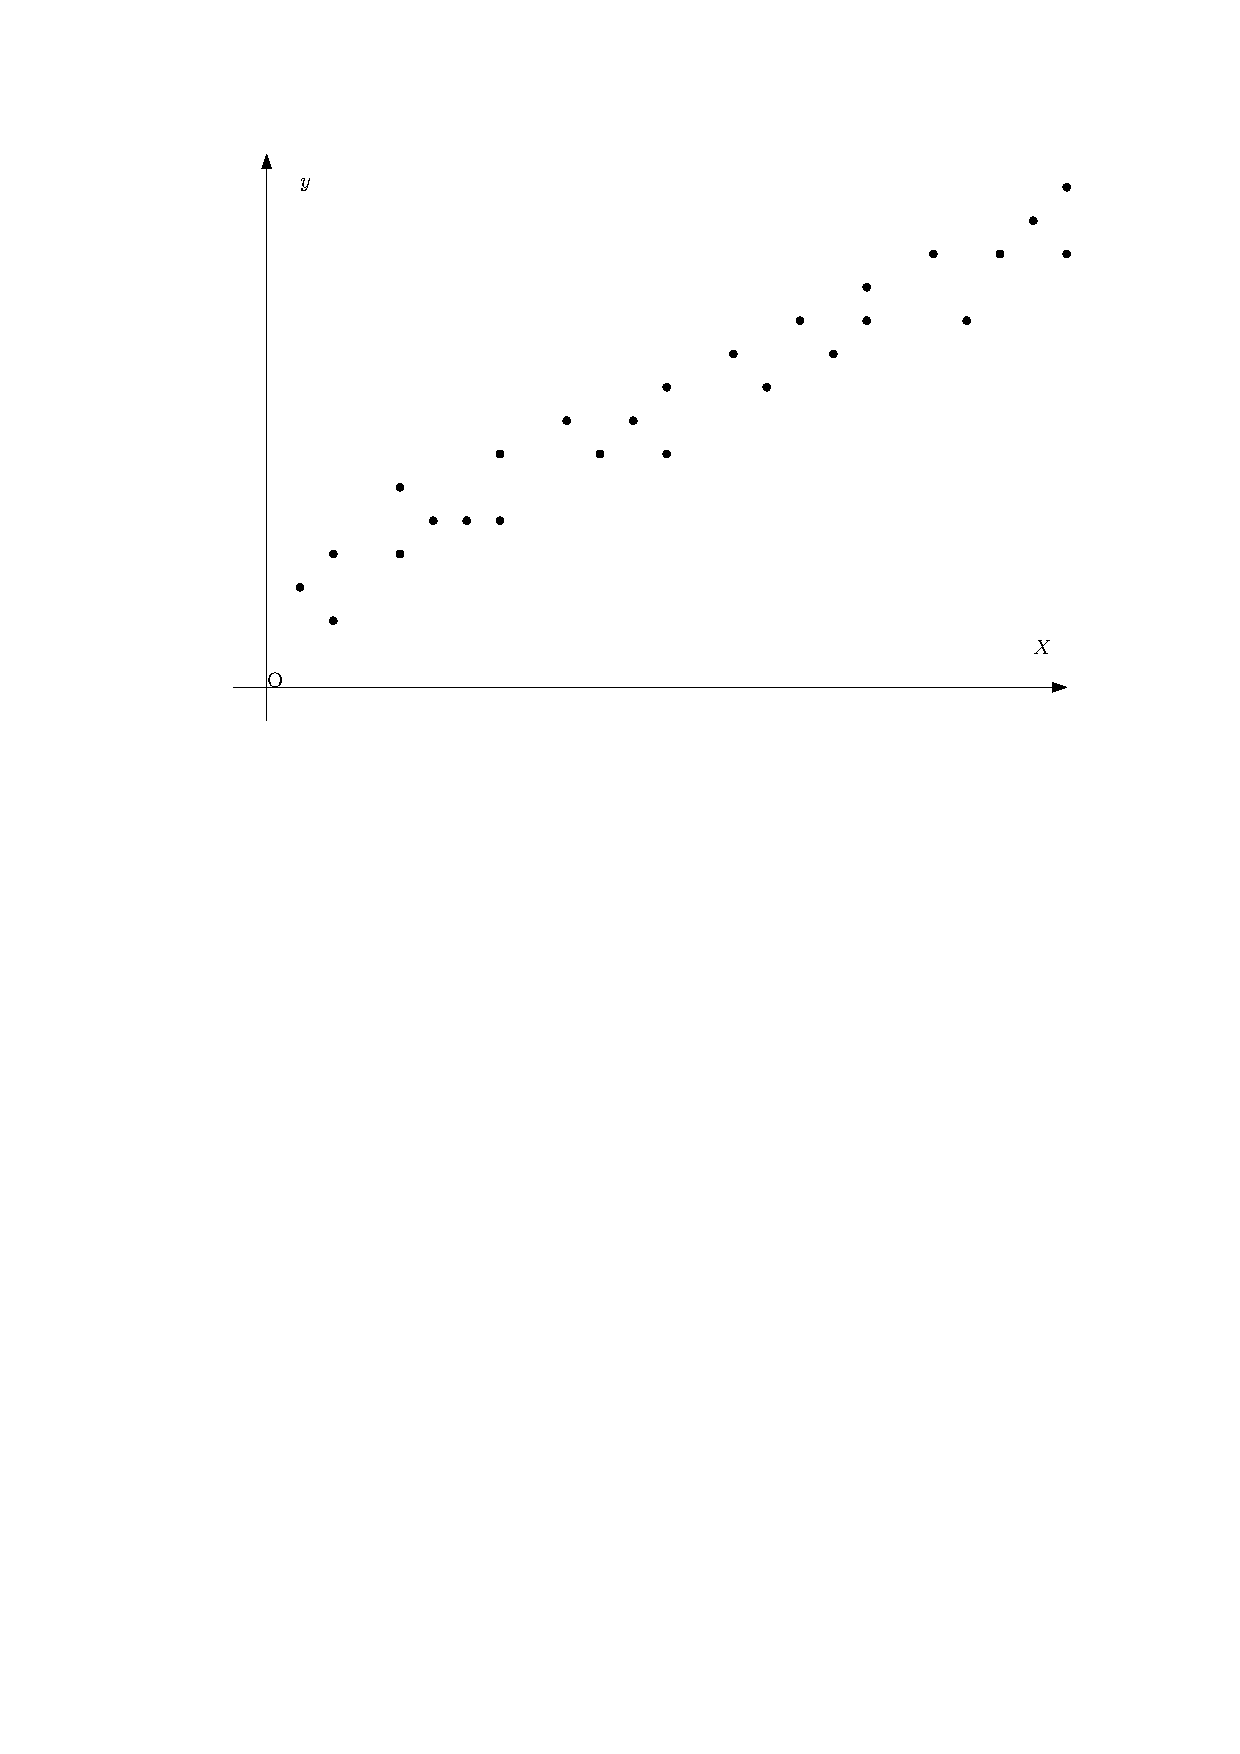
\includegraphics[width=.80\linewidth]{figure/whyML-analogy-1a.pdf}
            \caption{Simple Problem}
        \end{subfigure}
        \begin{subfigure} [b] {0.47\textwidth}
            \centering
            \phantom{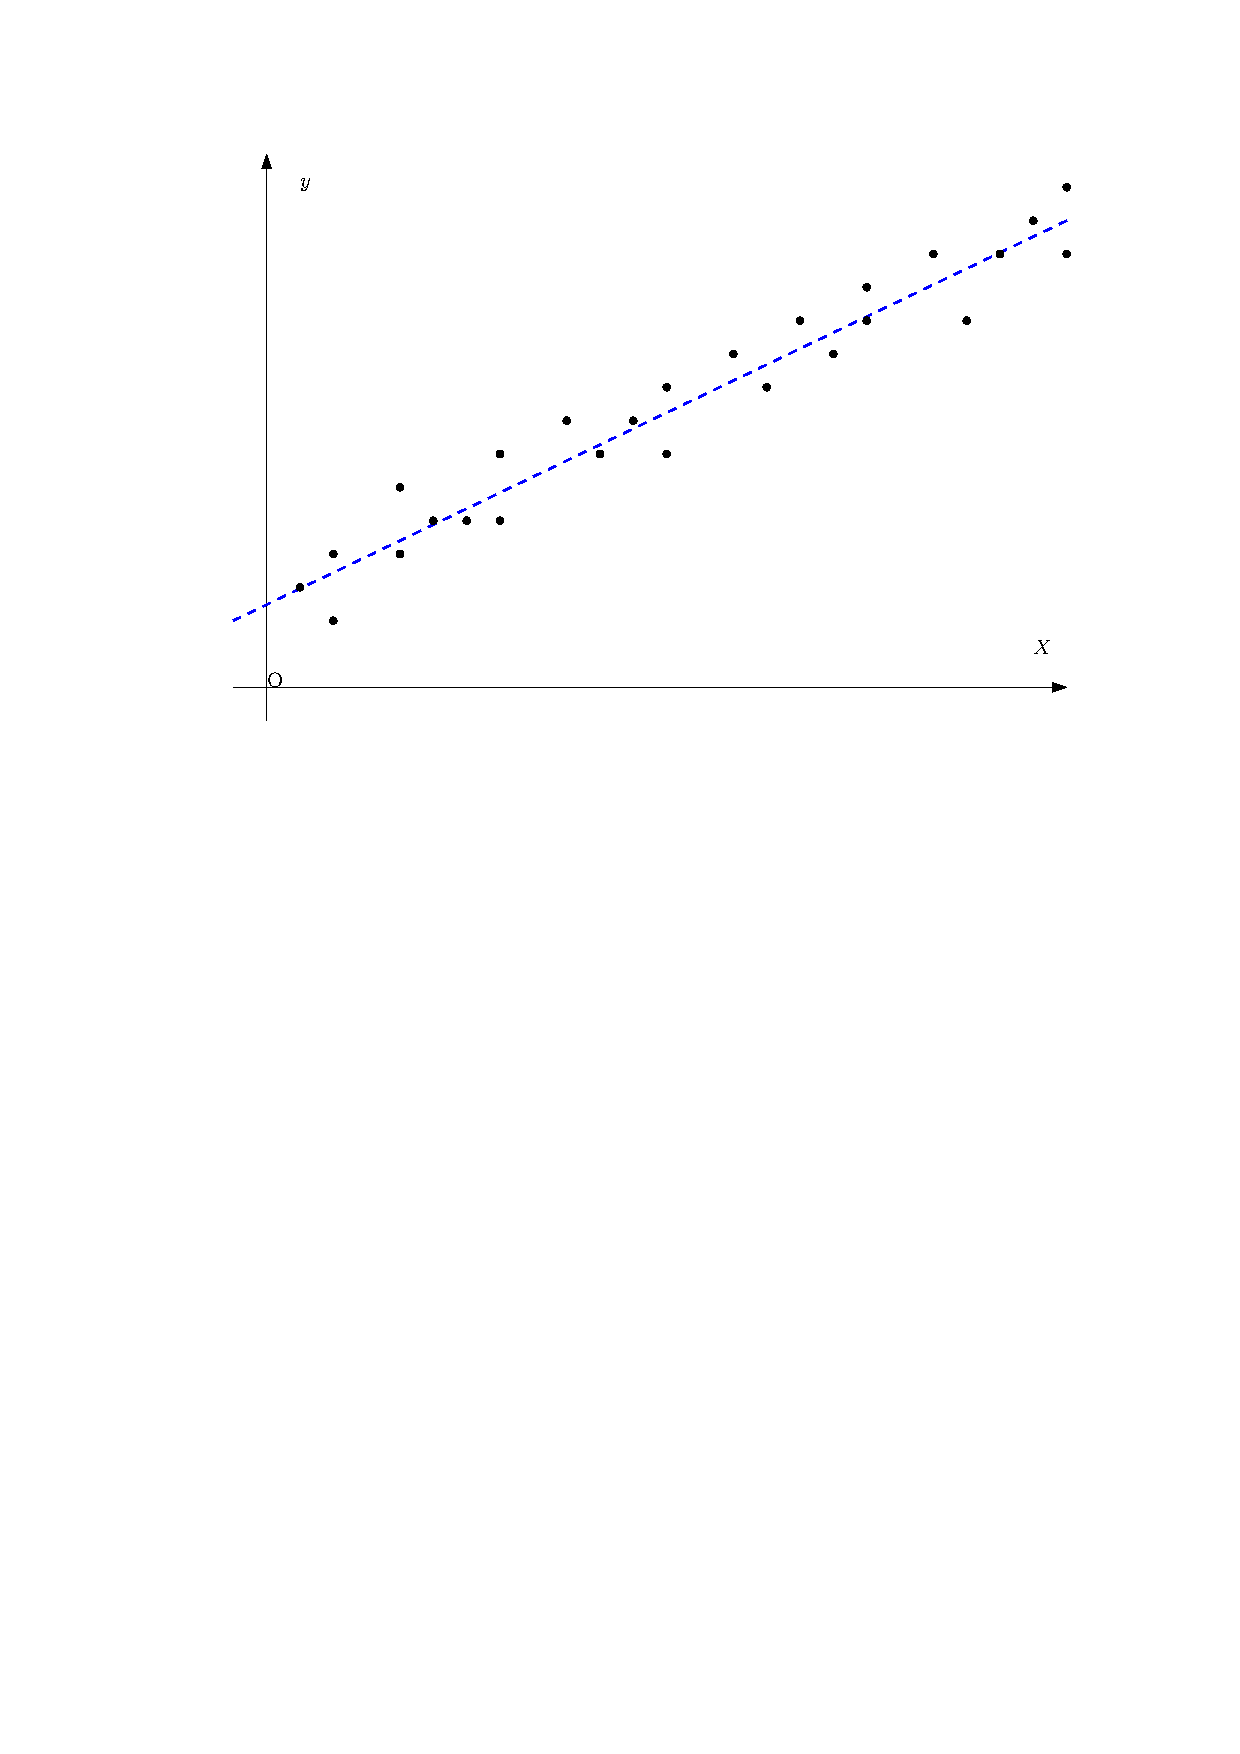
\includegraphics[width=.80\linewidth]{figure/whyML-analogy-1b.pdf}}
            \caption{Linear Regression (Simple)}
        \end{subfigure}
    \end{figure}
\end{frame}

\begin{frame}{Simple Puzzle (with linear regression)}
    \begin{figure}[H]
        \centering
        \begin{subfigure} [b] {0.47\textwidth}
            \centering
            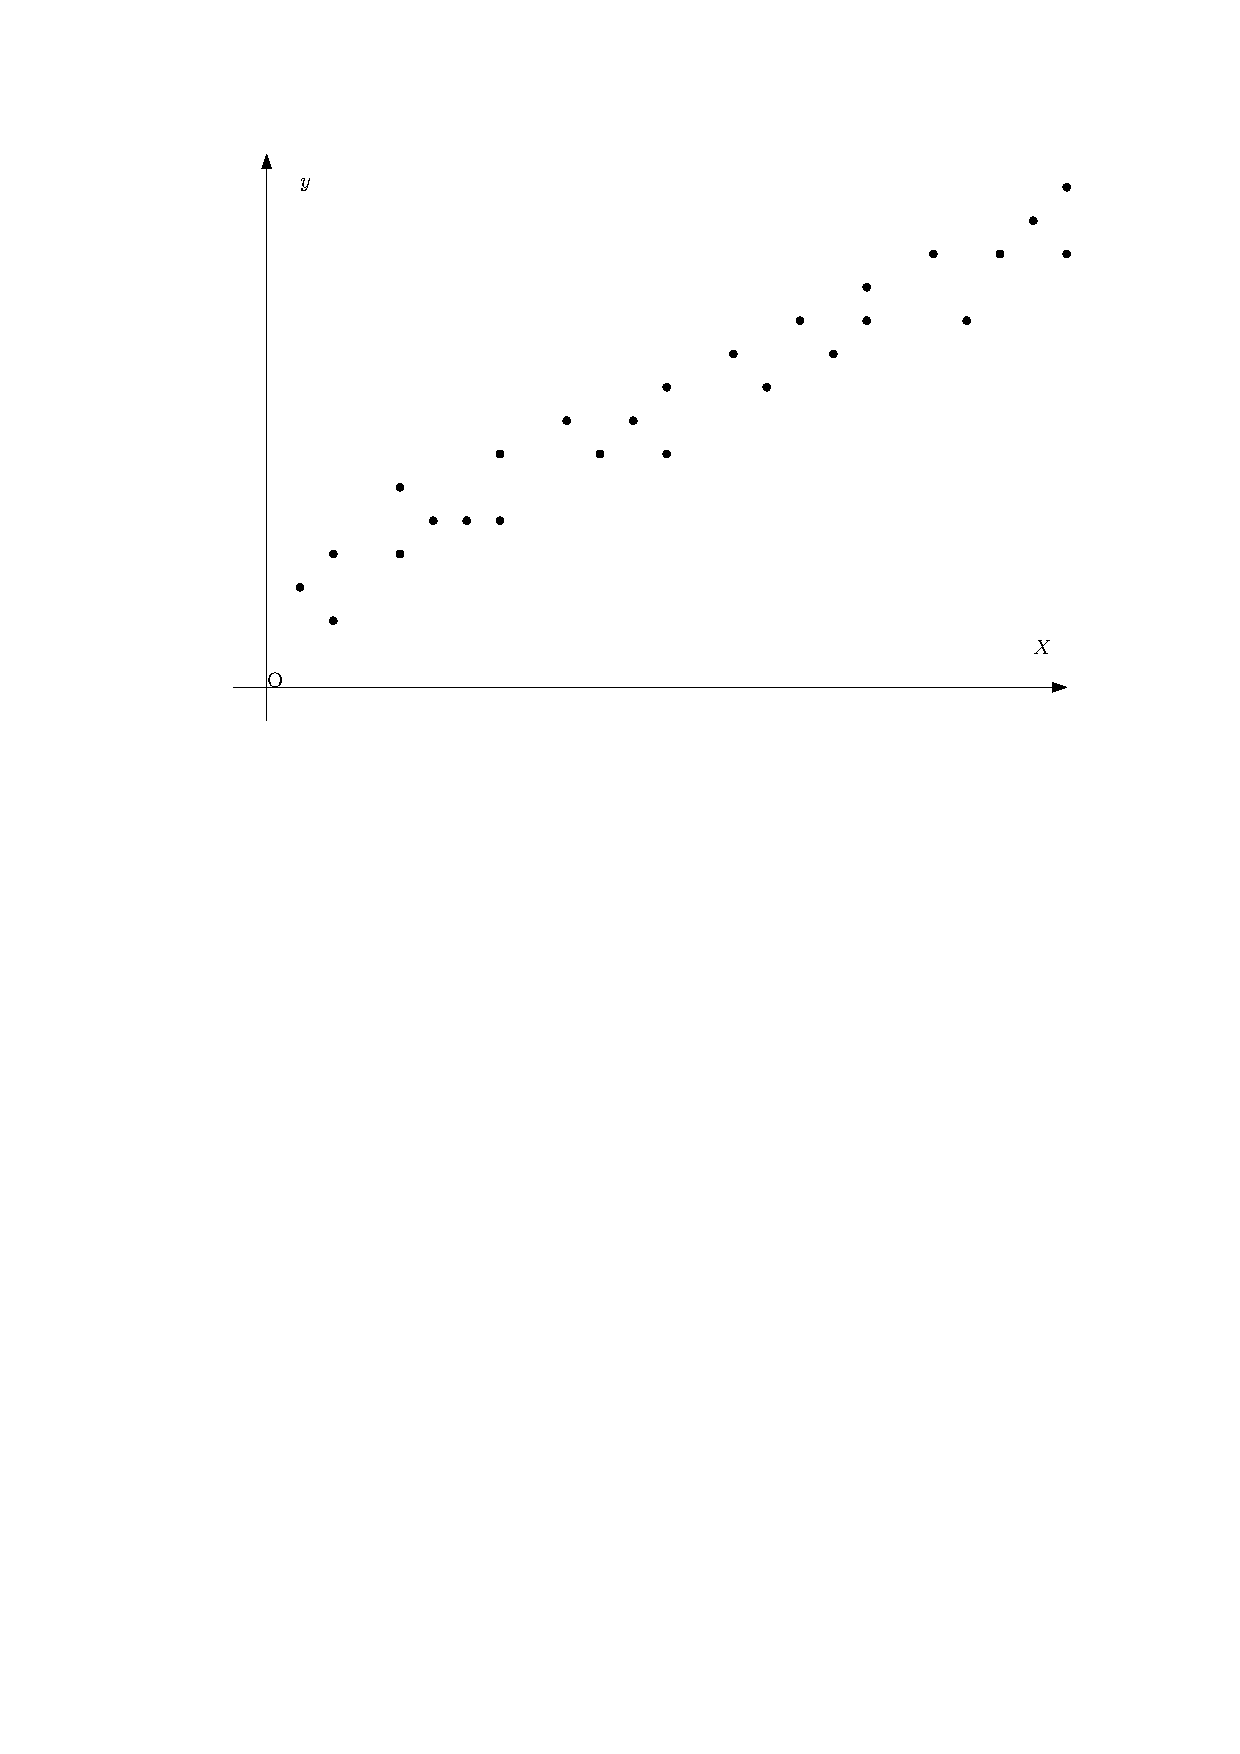
\includegraphics[width=.80\linewidth]{figure/whyML-analogy-1a.pdf}
            \caption{Simple Problem}
        \end{subfigure}
        \begin{subfigure} [b] {0.47\textwidth}
            \centering
            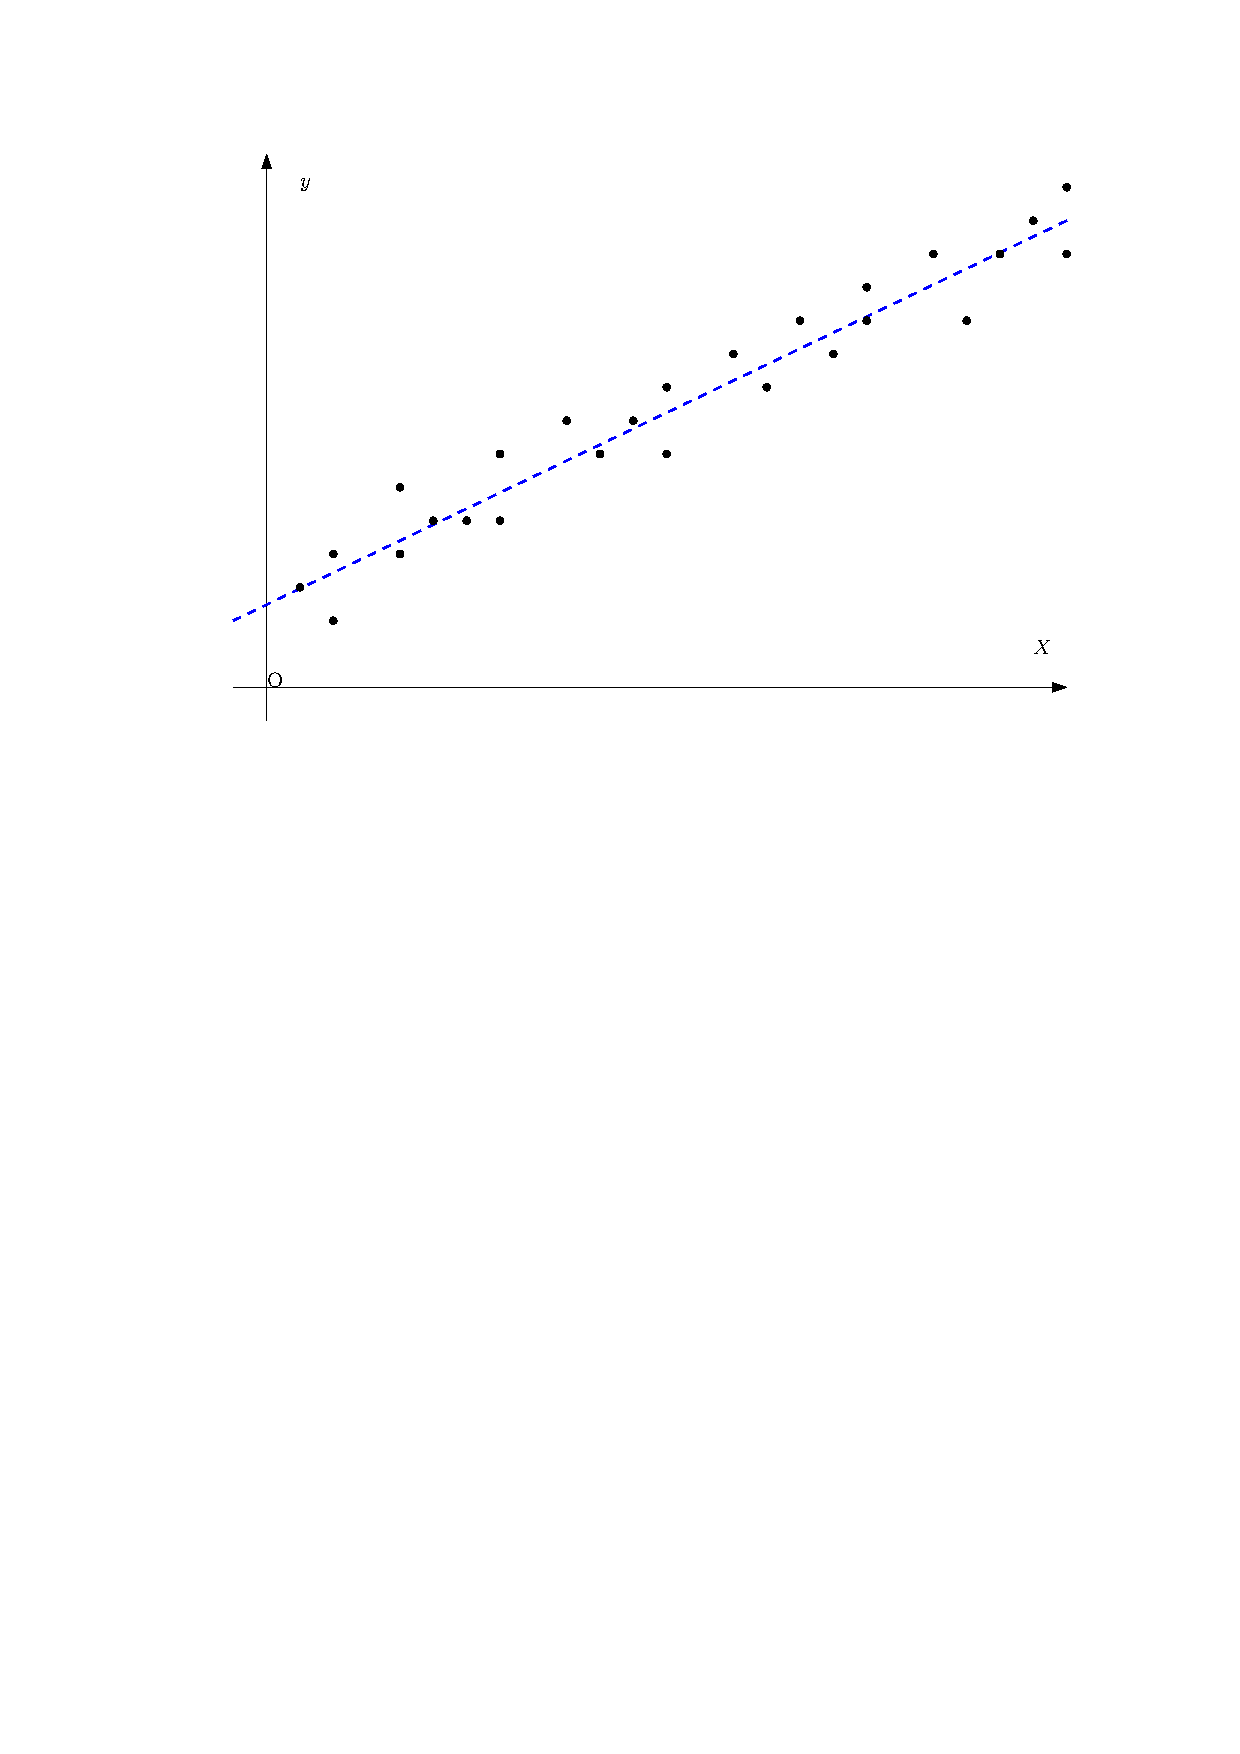
\includegraphics[width=.80\linewidth]{figure/whyML-analogy-1b.pdf}
            \caption{Linear Regression (Simple)}
        \end{subfigure}
    \end{figure}
\end{frame}

\begin{frame}{Complicated Puzzle (with Machine Learning)}
    \begin{figure}[H]
        \centering
        \begin{subfigure} [b] {0.47\textwidth}
            \centering
            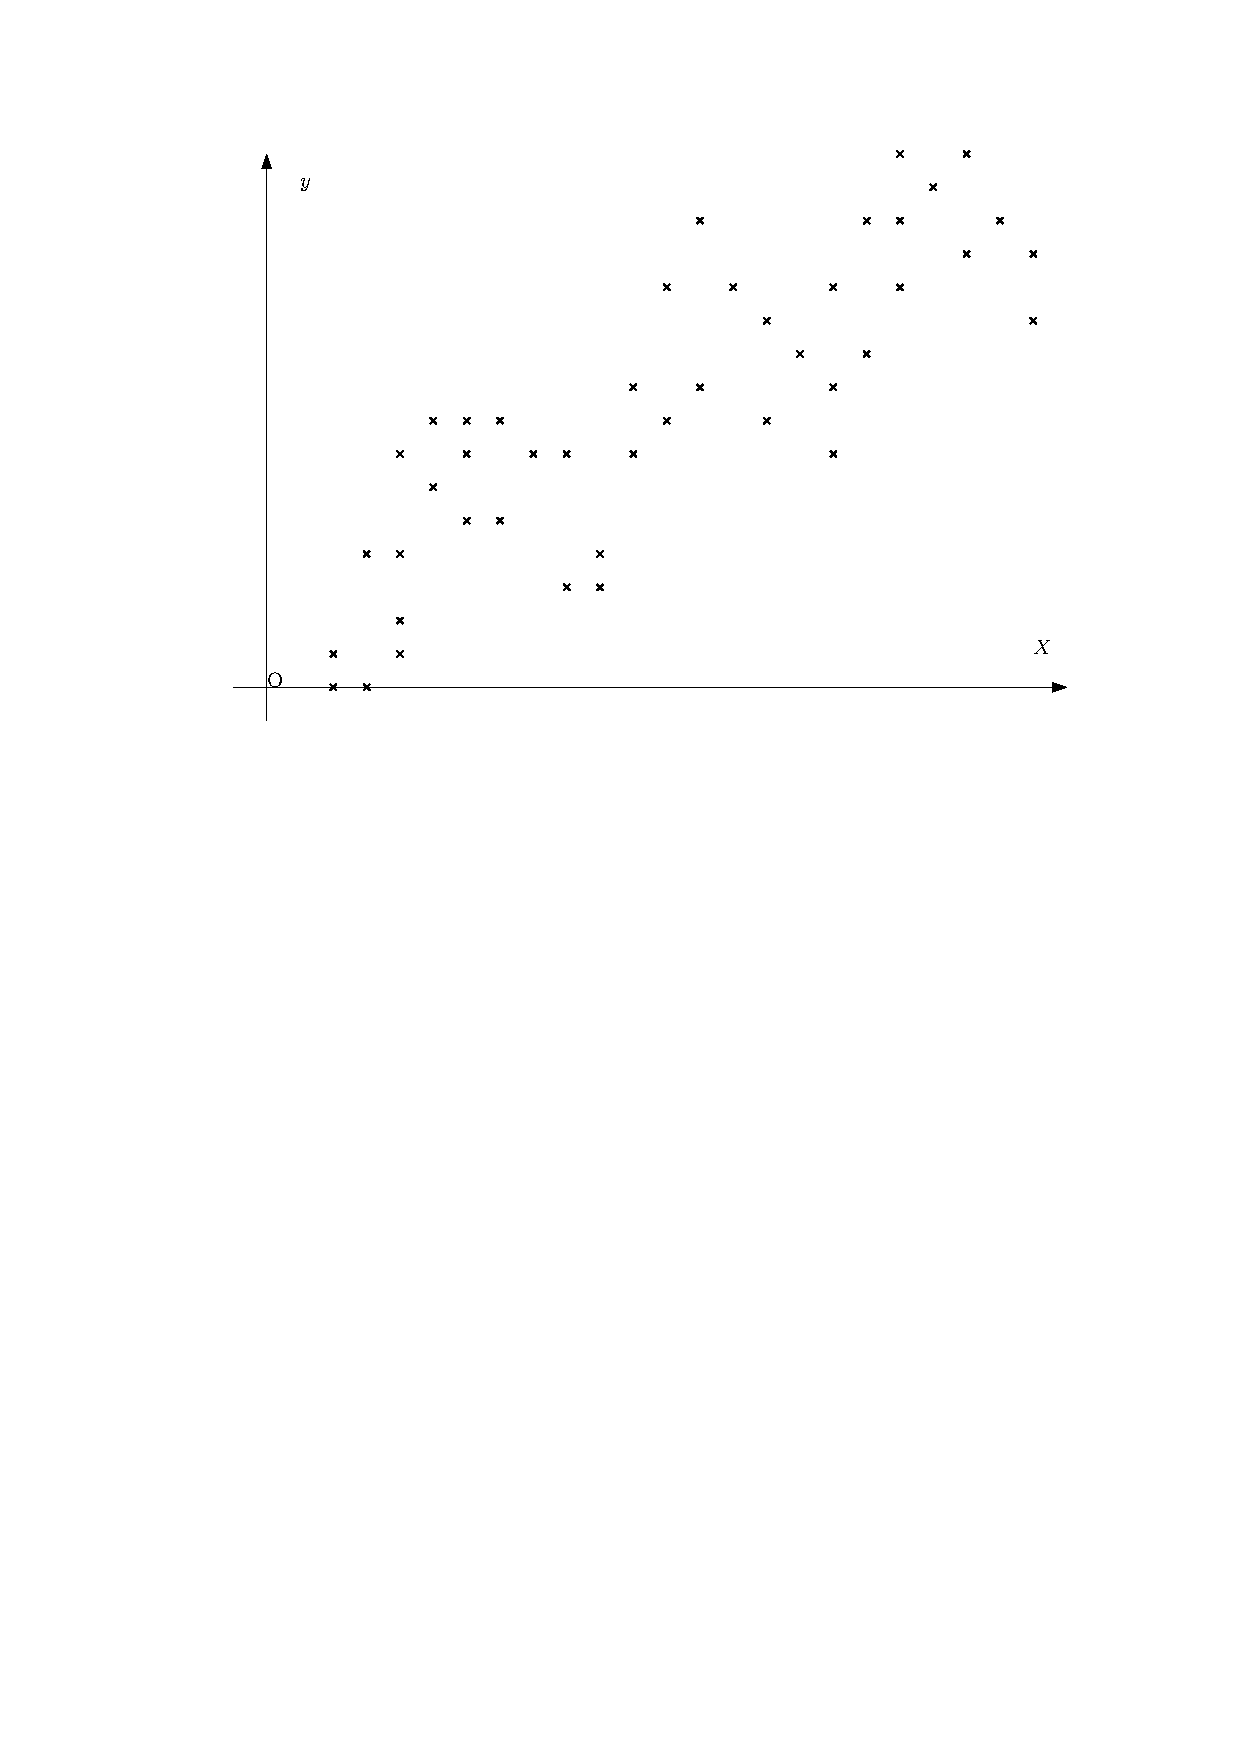
\includegraphics[width=.80\linewidth]{figure/whyML-analogy-2a.pdf}
            \caption{Complicated Problem}
        \end{subfigure}
        \begin{subfigure} [b] {0.47\textwidth}
            \centering
            \phantom{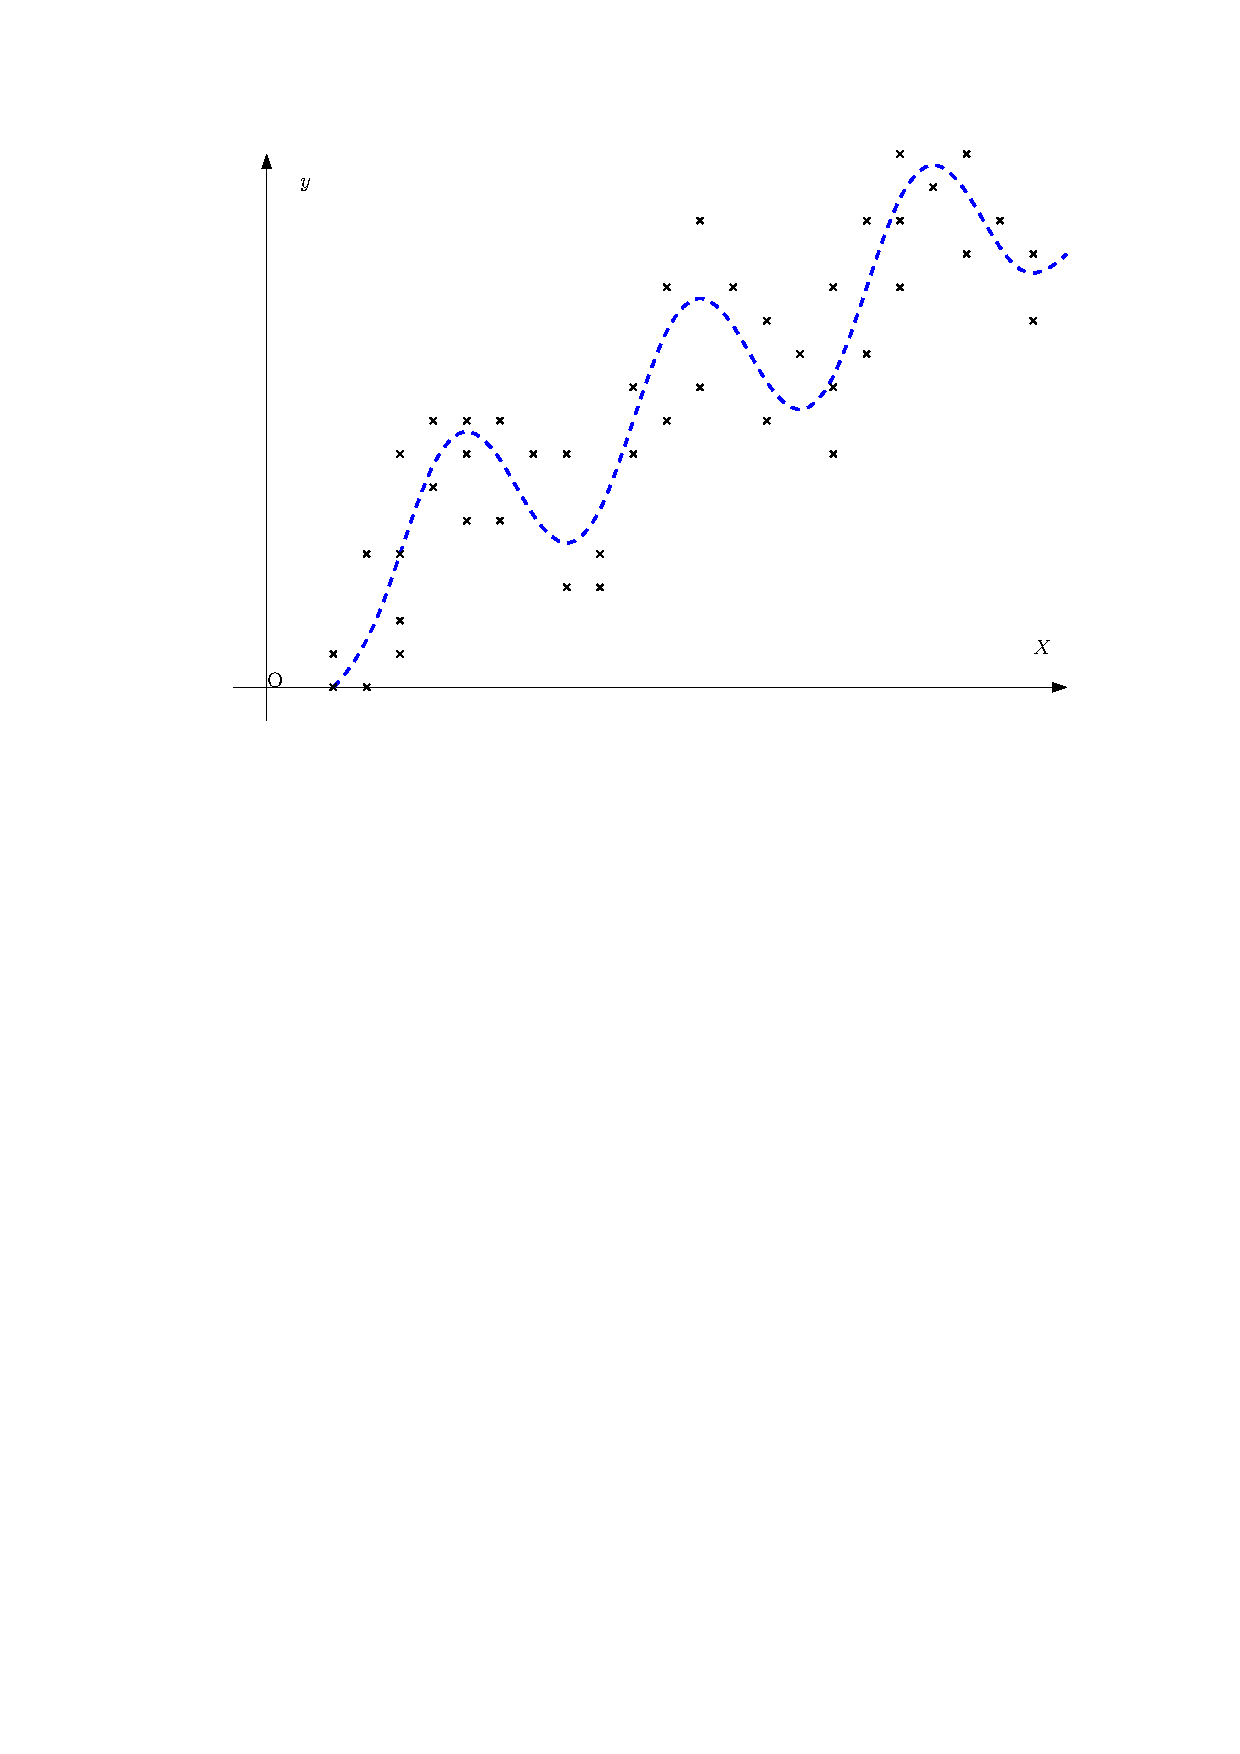
\includegraphics[width=.80\linewidth]{figure/whyML-analogy-2b.pdf}}
            \caption{Machine Learning (Complicated)}
        \end{subfigure}
    \end{figure}
\end{frame}

\begin{frame}{Complicated Puzzle (with Machine Learning)}
    \begin{figure}[H]
        \centering
        \begin{subfigure} [b] {0.47\textwidth}
            \centering
            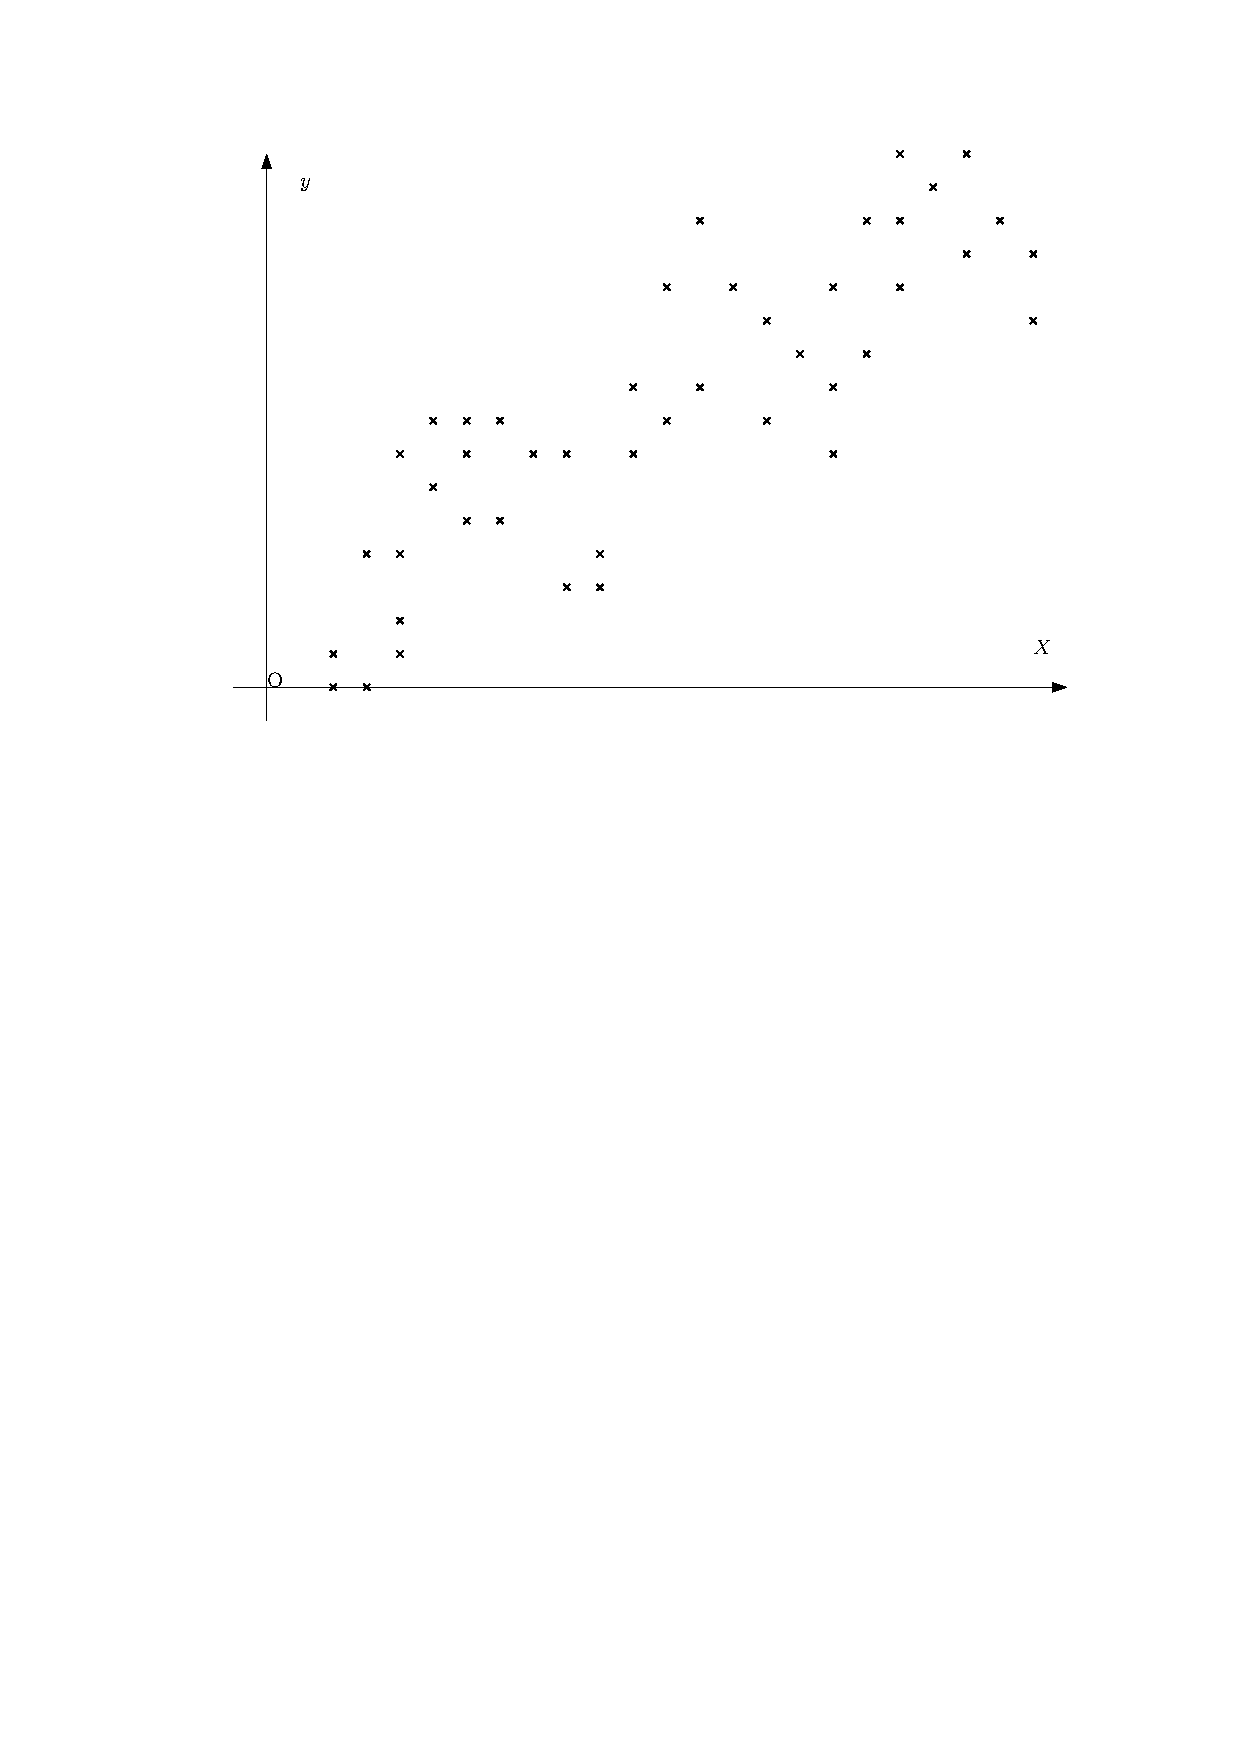
\includegraphics[width=.80\linewidth]{figure/whyML-analogy-2a.pdf}
            \caption{Complicated Problem}
        \end{subfigure}
        \begin{subfigure} [b] {0.47\textwidth}
            \centering
            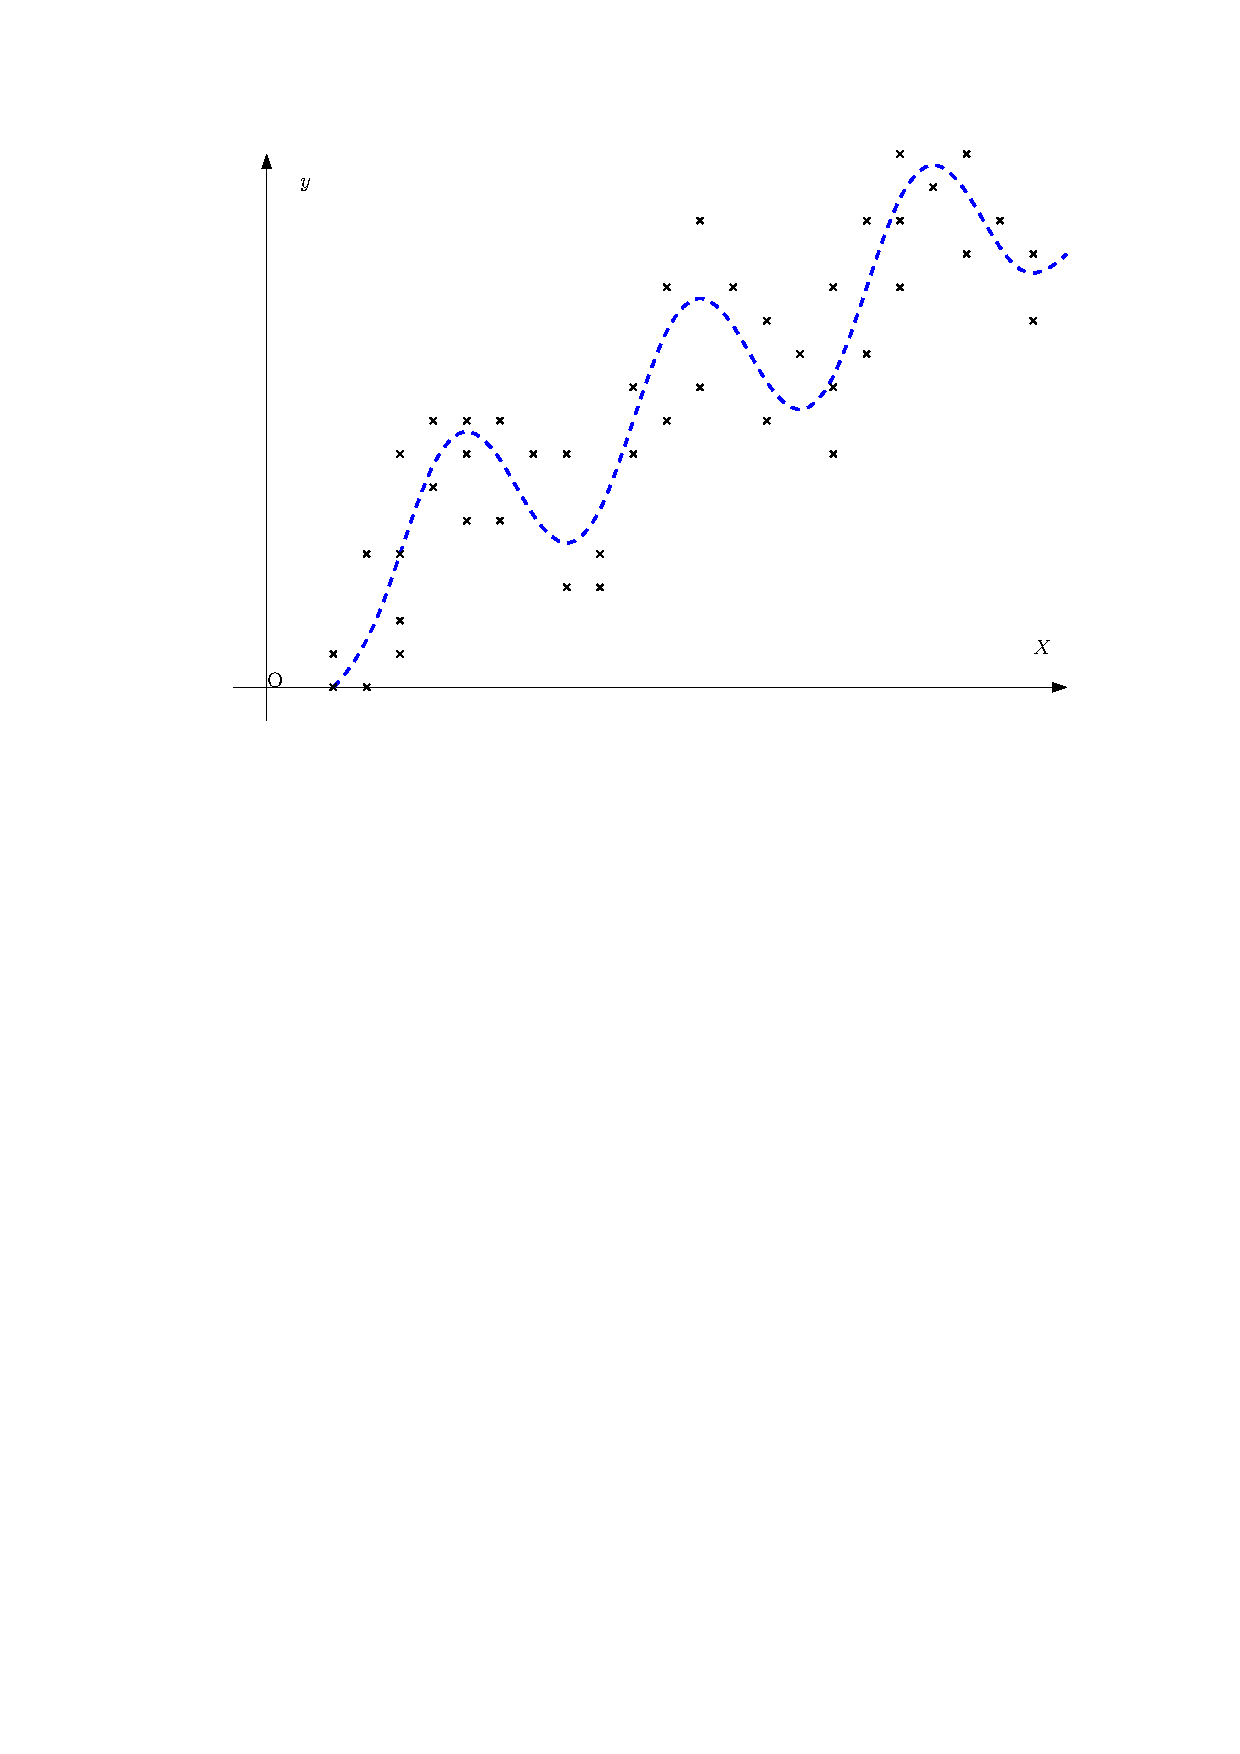
\includegraphics[width=.80\linewidth]{figure/whyML-analogy-2b.pdf}
            \caption{Machine Learning (Complicated)}
        \end{subfigure}
    \end{figure}
\end{frame}

% \begin{frame}{Background}
%     \begin{block}{Key Concept}
%         Place a definition or important concept here~\cite{book:571187}.
%     \end{block}

%     \begin{alertblock}{Warning}
%         Use alert blocks to draw attention.
%     \end{alertblock}
% \end{frame}

% ==================================================
\section{Experiences}
\title[3/4 Experiences]
% ==================================================

\begin{frame}{Problem}
    \begin{block}{Problem}
        집의 여러 정보를 기반으로 집값을 예측하는 모델 만들기.
    \end{block}

\end{frame}

\begin{frame}{Problem}
    \begin{block}{Problem}
        집의 여러 정보를 기반으로 집값을 예측하는 모델 만들기.
    \end{block}
    
    \begin{columns}
        \begin{column}[t]{0.48\textwidth}
            \begin{itemize}
                \item 데이터: 1168개 % train: 1460=1168(train)+292(validation), test: 1459
                \item X값(columns): 36가지 ($MasVnrArea, GarageYrBlt, LotFrontage, \dots$)
                \item y값 : 가격
            \end{itemize}
        \end{column}

        \begin{column}[t]{0.48\textwidth}
            \begin{table}
                \centering
                \begin{tabular}{lc}
                    \toprule
                    LotFrontage & 212 \\
                    MasVnrArea & 6 \\
                    GarageYrBlt & 58 \\
                    \bottomrule
                \end{tabular}
                \caption{number of missing values}
            \end{table}
        \end{column}
    \end{columns}

    \begin{alertblock}{Core Problem}
        How do I handle the missing data?
    \end{alertblock}
\end{frame}

% 대충 imputing, dropping 등에 대한 설명 with figure
% \begin{frame}{Experiment}
%     \begin{table}
%         \centering
%         \begin{tabular}{lccc|c}
%             \toprule
%             Exp \# & $MasVnrArea$ & $GarageYrBlt$ & $LotFrontage$ & MSE (Error) \\
%             \midrule
%             Baseline 1 & DROP & DROP & DROP & 17837.82570776256 \\
%             Baseline 2 & IMP & IMP & IMP & 18062.894611872147 \\
%             Exp 1 & IMP & IMP & DROP & 18105.497933789953 \\
%             Exp 2 & IMP & DROP & IMP & \textbf{17809.983767123285} \\
%             \bottomrule
%         \end{tabular}
%         \caption{Comparison of methods.}
%     \end{table}
% \end{frame}

\begin{frame}{Experiment}
    \begin{table}
        \centering
        \begin{tabular}{lccc|c}
            \toprule
            Exp \# & $MasVnrArea$ & $GarageYrBlt$ & $LotFrontage$ & MSE (Error) \\
            \midrule
            Baseline 1 & DROP & DROP & DROP & 17837.82570776256 \\
            Baseline 2 & IMP & IMP & IMP & 18062.894611872147 \\
            Exp 1 & IMP & IMP & DROP & 18105.497933789953 \\
            Exp 2 & IMP & DROP & IMP & \textbf{17809.983767123285} \\
            \bottomrule
        \end{tabular}
        \caption{Comparison of methods.}
    \end{table}
\end{frame}

% ==================================================
\section{Insights}
\title[4/4 Insights]
% ==================================================



% \begin{frame}{한국어 (kotex) 테스트}
%     \begin{block}{kotex 동작 확인}
%         이 슬라이드는 \texttt{kotex} 패키지가 정상적으로 동작하는지 확인합니다.
%     \end{block}

%     \begin{itemize}
%         \item 가나다라마바사 — 기본 한글 자모
%         \item \textbf{굵은 글씨}와 \hangulit{기울임꼴} 지원
%         \item 숫자 및 혼용: 2024년 1월 1일
%         \item 영문 혼용: LuaLaTeX으로 컴파일된 한국어 슬라이드
%     \end{itemize}

%     \begin{alertblock}{주의사항}
%         한글 폰트가 시스템에 설치되어 있어야 합니다.
%         기본값은 \texttt{kotex}가 자동으로 선택합니다.
%     \end{alertblock}
% \end{frame}

% ==================================================
\section{Conclusion}
% ==================================================

\begin{frame}{Conclusion}
    \begin{enumerate}
        \item Summary point one.
        \item Summary point two.
        \item Future work direction.
    \end{enumerate}
\end{frame}

\begin{frame}[allowframebreaks]{References}
    \bibliographystyle{plain}
    \bibliography{refs}
\end{frame}

\end{document}
